The results of the experiments are presented in Figures \ref{fig:results-deviations} and 3, and Tables \ref{tab:average-results} and \ref{tab:significance-tests}.

The primary metric used to compare the results of the algorithms is average percentage deviation from the best known solution for each problem.
This is determined by first calculating the percentage deviation of each trial result using the expression,
\[
    100\left(\frac{(\text{trial solution})- (\text{best known solution})}{(\text{best known solution})}\right)\%,
\]
then computing the mean deviation across all repetitions of each trial.

Each algorithm was run on each problem instance in the QAPLIB 12 times, and the average percentage deviation from the best known value (BKV), the percentage of runs on which the BKV, and the average time to find the BKV were recorded for each instance and algorithm.

Table~\ref{tab:average-results} presents the average results achieved by each algorithm averaged over the set of QAPLIB problems.
It is clear from the table that the BMA algorithm found the best known value on the greatest percentage of attempts, and the solutions it returned had the lowest average deviation from the best known values.
The second most effective method was ITS, as measured by both of the same metrics, followed by simulated annealing and the simple evolutionary algorithm.
The Wilcoxon signed rank test results presented in Table~\ref{tab:significance-tests} confirms this ordering, with a significance of \(p<0.001\) in every case.

\begin{table}[h]
    \centering
    \caption{Experiment results for each algorithm averaged over all QAPLIB problems.}
    \label{tab:average-results}
    \begin{tabularx}{0.74\textwidth}{@{}l|rrr@{}}
        \toprule
        Algorithm & Deviation (\%) & BKV Time (s) & \% BKV Solutions \\
        \midrule
        SA  &  6.37 & 5.62 & 25.43 \\
        ITS &  3.10 & 0.88 & 28.23 \\
        BMA &  0.61 & 0.69 & 68.92 \\
        EA  & 11.33 & 0.66 & 10.19 \\
        \bottomrule
    \end{tabularx}
\end{table}

\begin{table}[h]
    \centering
    \caption{Wilcoxon signed rank tests on the average percentage deviations from the BKV}
    \label{tab:significance-tests}
    \begin{tabularx}{0.29\textwidth}{@{}ll|r@{}}
        \toprule
        \multicolumn{2}{c}{Algorithms} & p-value \\
        \midrule
        BMA & ITS & \(<0.0001\) \\ % V = 434
        BMA & EA  & \(<0.0001\) \\ % V = 0
        BMA & SA  & \(<0.0001\) \\ % V = 65
        ITS & EA  & \(<0.0001\) \\ % V = 448
        ITS & SA  & \( 0.0004\) \\ % V = 2537
        EA  & SA  & \(>0.9999\) \\ % V = 7374
        % alternative hypothesis: true location shift is less than 0
        \bottomrule
    \end{tabularx}
\end{table}

Figure~\ref{fig:results-deviations} presents a box plot of the distributions of the average percentage deviations that each algorithm attained across the problem instances in the QAPLIB.
The length of whiskers of each box in the figure are restricted to 1.5 times the interquartile range of the corresponding distribution. Points outside of this range are drawn as outliers.
The range of deviations in the plot is restricted to \([0\%, 30\%]\), as the maximum deviations returned by the evolutionary algorithm and simulated annealing were as high as 156\% and 237\% respectively.
The maximum attained returned by BMA was 17\%, and the maximum deviation attained by ITS was 33\%.
It is clear that the medians, and variances of the distribution of deviations attained by each algorithm follow a similar ordering as the mean deviations and number of BKV solutions found.

Figure~3 presents the distribution of deviations attained by each algorithm on a partition of the QAPLIB instances into problems of size greater than 50 (\scarequotes{large} problems), and those that were not (\scarequotes{small} problems).
The means medians and variances for both small and large problems follow the ordering previously established between algorithms.
The distributions of deviations for small problems are very similar to those of the total problem set.
However, the distributions of deviations for the large problems are quite different. In particular, the mean and median of the results for simulated annealing and for the evolutionary algorithm are higher, and the variances of the distributions are larger.

\begin{figure}
    \centering
    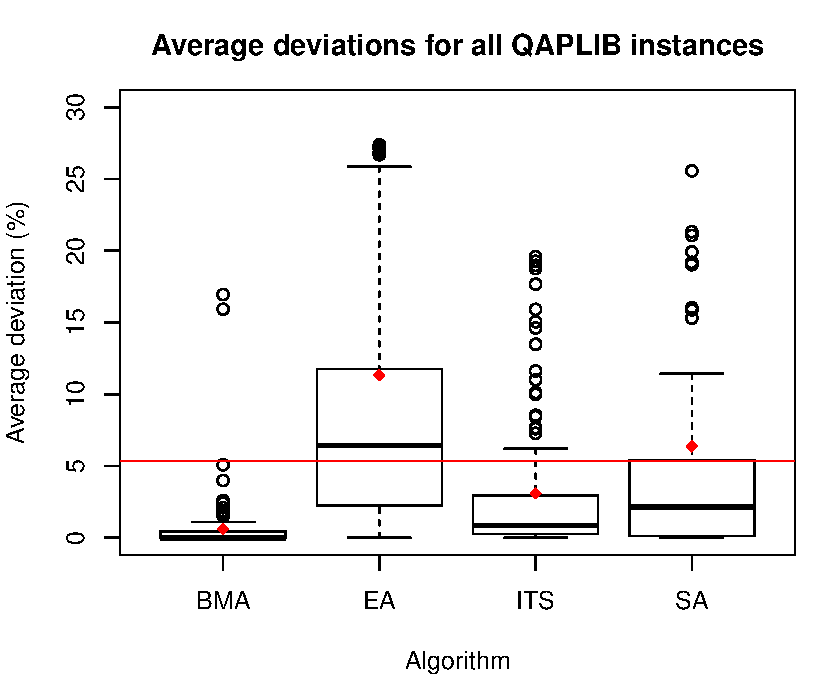
\includegraphics[width=0.75\textwidth]{figures/results-deviations-box-plot.pdf}%
    \caption{
        Box plots of the distribution of average deviations attained over the QAPLIB instances by each of the four methods.
        The length of whiskers of each box in the figure are restricted to 1.5 times the interquartile range of the corresponding distribution. Points outside of this range are drawn as outliers.
        The red points and red line represent the means of each distribution and the overall mean, respectively.
    }
    \label{fig:results-deviations}

    \vspace{1cm}

    \begin{tabularx}{\textwidth}{@{}lr@{}}
        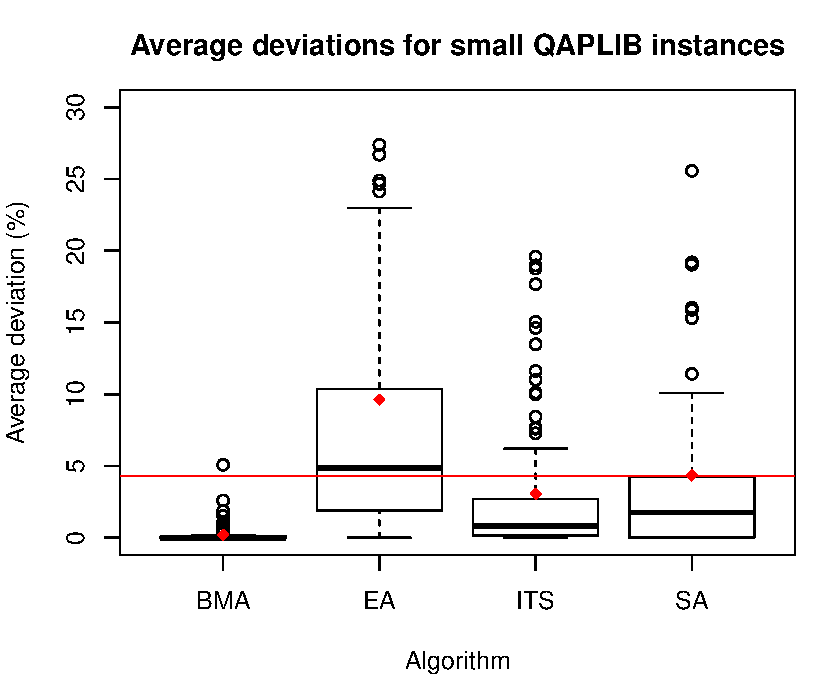
\includegraphics[width=0.5\textwidth]{figures/results-deviations-small-box-plot.pdf} &
        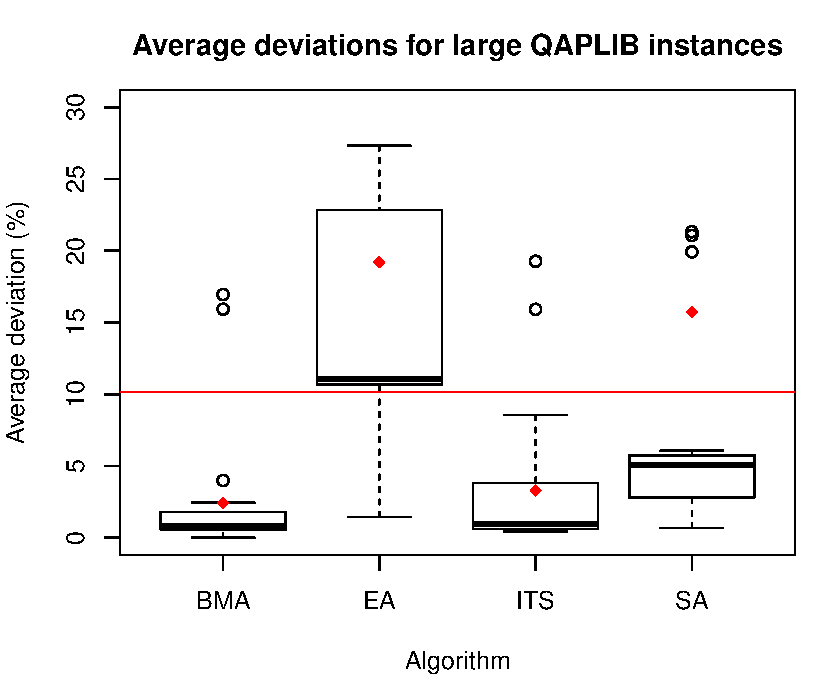
\includegraphics[width=0.5\textwidth]{figures/results-deviations-large-box-plot.pdf}
    \end{tabularx}
    \caption{
        Box plots of the distribution of average deviations attained over the QAPLIB instances by each of the four methods.
        The instances have been partitioned into problems of size greater than 50 (\scarequotes{large} problems), and those that were not (\scarequotes{small} problems).
    }
    \label{tab:results-deviations-types}
\end{figure}


    % \begin{figure}
    %     \centering
    %     \begin{tabularx}{\textwidth}{@{}lr@{}}
    %         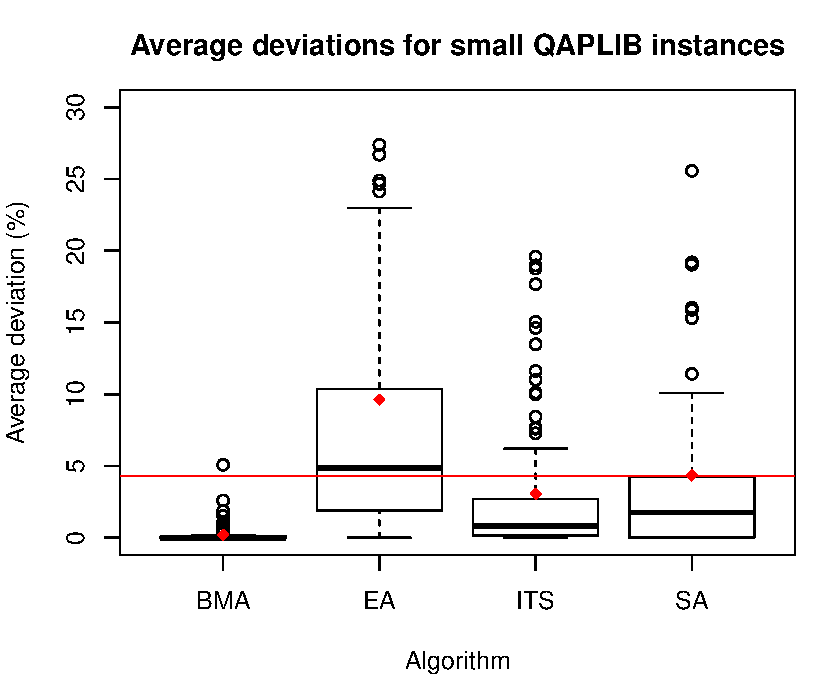
\includegraphics[width=0.5\textwidth]{figures/results-deviations-small-box-plot.pdf} &
    %         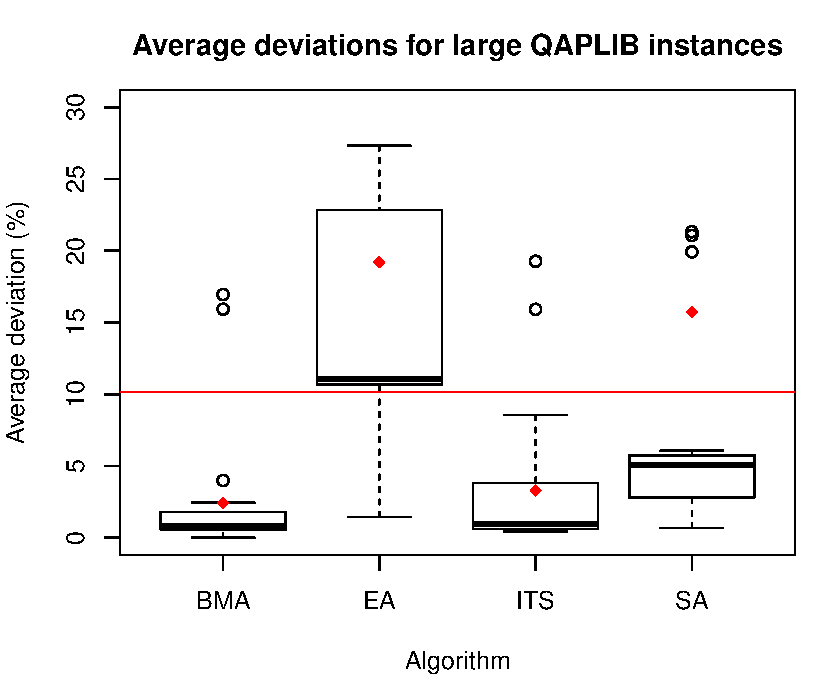
\includegraphics[width=0.5\textwidth]{figures/results-deviations-large-box-plot.pdf}
    %     \end{tabularx}
    %     \caption{\todo{Caption}}
    %     \label{tab:results-deviations-types}
    % \end{figure}

% \subsection{Significance tests} {
    % Wilcoxon signed rank tests on the \% deviation from the BKV:

        % \begin{tabularx}{0.29\textwidth}{@{}ll|r@{}}
        %     \toprule
        %     \multicolumn{2}{c}{Algorithms} & p-value \\
        %     \midrule
        %     BMA & ITS & \(>0.9999\) \\ % V = 434
        %     BMA & EA  & \(>0.9999\) \\ % V = 0
        %     BMA & SA  & \(>0.9999\) \\ % V = 65
        %     ITS & EA  & \(>0.9999\) \\ % V = 448
        %     ITS & SA  & \( 0.9996\)  \\ % V = 2537
        %     EA  & SA  & \(<0.0001\) \\ % V = 7374
        %     % alternative hypothesis: true location shift is greater than 0
        %     \bottomrule
        % \end{tabularx}
    % \end{table}
% }

% \subsection{Discussion} {
%
% }
